\section{Factored Variation Approximation}

\begin{remark}{\textbf{(Intractable EM-Method)}}
    Sometime E-step or M-step are intractable; therefore, we will have to do some approximation to the problem:
    \begin{itemize}
        \item It might be the case that $P(\mathcal{Z} | \mathcal{X}, \theta)$ and so we might replace M-step with gradient M-step, where every step increase the likelihood.
        \item In E-step, we should consider parameterized $q = q(\mathcal{Z})$ and take the gradient step in $\rho$. 
        \item Or we assume some simplification for $q$ usually $q = \prod_iq_i(\mathcal{Z}_i)$ where $\mathcal{Z}_i$ is the partition $\mathcal{Z}$.
    \end{itemize}
\end{remark}

\begin{remark}{\textbf{(Restricting Variational Class)}}
    This approximation of E-step is the same as choosing $q$ from the limit set $\mathcal{Q}$ such that VE-step is to maximize $\mathcal{F}(q, \boldsymbol \theta)$ such that:
    \begin{equation*}
        q^{(k)}(\mathcal{Z}) = \argmax{q\in\mathcal{Q}}\mathcal{F}(q(\mathcal{F}), \boldsymbol \theta^{(k-1)})
    \end{equation*}
    The effect of the restricting $q$ to $\mathcal{Q}$, there is the following effect:
    \begin{itemize}
        \item The free energy is bounded by log-likelihood via Jensen's inequality as $\mathcal{F}(q, \boldsymbol \theta) \le l(\theta^\text{ML})$, thus as long as every step increases $\mathcal{F}$ convergence still guarantee. 
        \item Since $P(\mathcal{Z} | \mathcal{X}, \boldsymbol \theta^{(k)})$ may not lie in $Q$ and we no longer saturated the bound after E-step. The likelihood may not increase on each full EM step. 
    \end{itemize}
\end{remark}

\begin{definition}{\textbf{(Factored Variational E-Step)}}
    We consider the following family of distributions:
    \begin{equation*}
        \mathcal{Q} = \brackc{q \left| q(\mathcal{Z}) = \prod_i q_i(\mathcal{Z}_i) \right.}
    \end{equation*}
    where $\mathcal{Z}$ are partitioned into $\brackc{\mathcal{Z_i}}$. We consider the following maximization of the E-step:
    \begin{equation*}
        q^{(k)}_i (\mathcal{Z}_i) =\argmax{q_i(\mathcal{Z}_i)}\mathcal{F}\bracka{q_i(\mathcal{Z}_i)\prod_{j\ne i}q_j(\mathcal{Z}_j), \ \boldsymbol \theta^{(k-1)}}
    \end{equation*}
\end{definition}

\begin{proposition}
    We can show that:
    \begin{equation*}
        q_i(\mathcal{Z}_i) \propto \exp\brackd{\log P(\mathcal{X}, \mathcal{Z} | \boldsymbol \theta^{(k-1)})}_{\prod_{j\ne i}q_j(\mathcal{Z}_j)}
    \end{equation*}
\end{proposition}
\begin{proof}
    Given this, the free energy is given by:
    \begin{equation*}
    \begin{aligned}
        \mathcal{F}\bracka{q_i(\mathcal{Z}_i)\prod_{j\ne i}q_j(\mathcal{Z}_j), \ \boldsymbol \theta^{(k-1)}} &= \brackd{\log P(\mathcal{X}, \mathcal{Z} | \boldsymbol \theta^{(k-1)})}_{\prod_jq_j(\mathcal{Z})} + H\brackb{\prod_j q_j(\mathcal{Z}_j)} \\
        &= \int q_i(\mathcal{Z}_i)\brackd{\log P(\mathcal{X}, \mathcal{Z} | \boldsymbol \theta^{(k-1)})}_{\prod_{j\ne i}q_j(\mathcal{Z}_j)}\dby \mathcal{Z}_i  + H[q_i] + \sum_{j\ne i}H[q_j]
    \end{aligned}
    \end{equation*}
    We will consider derivative of the Lagragian with normalizer of $q_i$, then we have:
    \begin{equation*}
        \frac{\partial}{\partial q_i}\bracka{\mathcal{F} + \lambda\bracka{\int q_i - 1}} = \brackd{\log P(\mathcal{X}, \mathcal{Z} | \boldsymbol \theta^{(k-1)})}_{\prod_{j\ne i}q_j(\mathcal{Z}_j)} - \log q_i(\mathcal{Z}_i) - \frac{q_i(\mathcal{Z}_i)}{q_i(\mathcal{Z}_i)} + \lambda =0
    \end{equation*}
    This implies that we have the update as defined above.
\end{proof}

\begin{remark}{\textbf{(Observations on Update Rule)}}
    This update of factorized model depends on the expected sufficient stistics of $q$ and this means that we don't need the entire distribution and just relevant expaction. If $\mathcal{Z}_i = z_i$ (factorized over all variables) then this technique is called mean field expectation:
    \begin{itemize}
        \item Suppose $P(\mathcal{X},\mathcal{Z})$ has sufficient statistics that are separated in the latent variables (for example Bolzman machine):
        \begin{equation*}
            P(\mathcal{X}, \mathcal{Z}) = \frac{1}{Z}\exp\bracka{\sum_{ij}W_{ij}s_is_j + \sum_ib_is_i}
        \end{equation*}
        \item The expectation with respected to fully factored $q$ over $z_i \in \mathcal{Z}$ gives us:
        \begin{equation*}
            \brackd{\log P(\mathcal{X}, \mathcal{Z})}_{\prod_i q_i} = \sum_{ij}W_{ij}\brackd{s_i}_{q_i}\brackd{s_j}_{q_j} +  \sum_{i}b_i\brackd{s_i}_{q_i}
        \end{equation*}
    \end{itemize}
    The update each $q_i$ given sufficient statistics of the other. Each variables see the mean field imposed by its neighbour and we update these fields until they all agree.
\end{remark}

\begin{remark}{\textbf{(Factored Variational Inference in Time Series)}}
    Consider the graphical model:
    \begin{figure}[H]
        \centering
        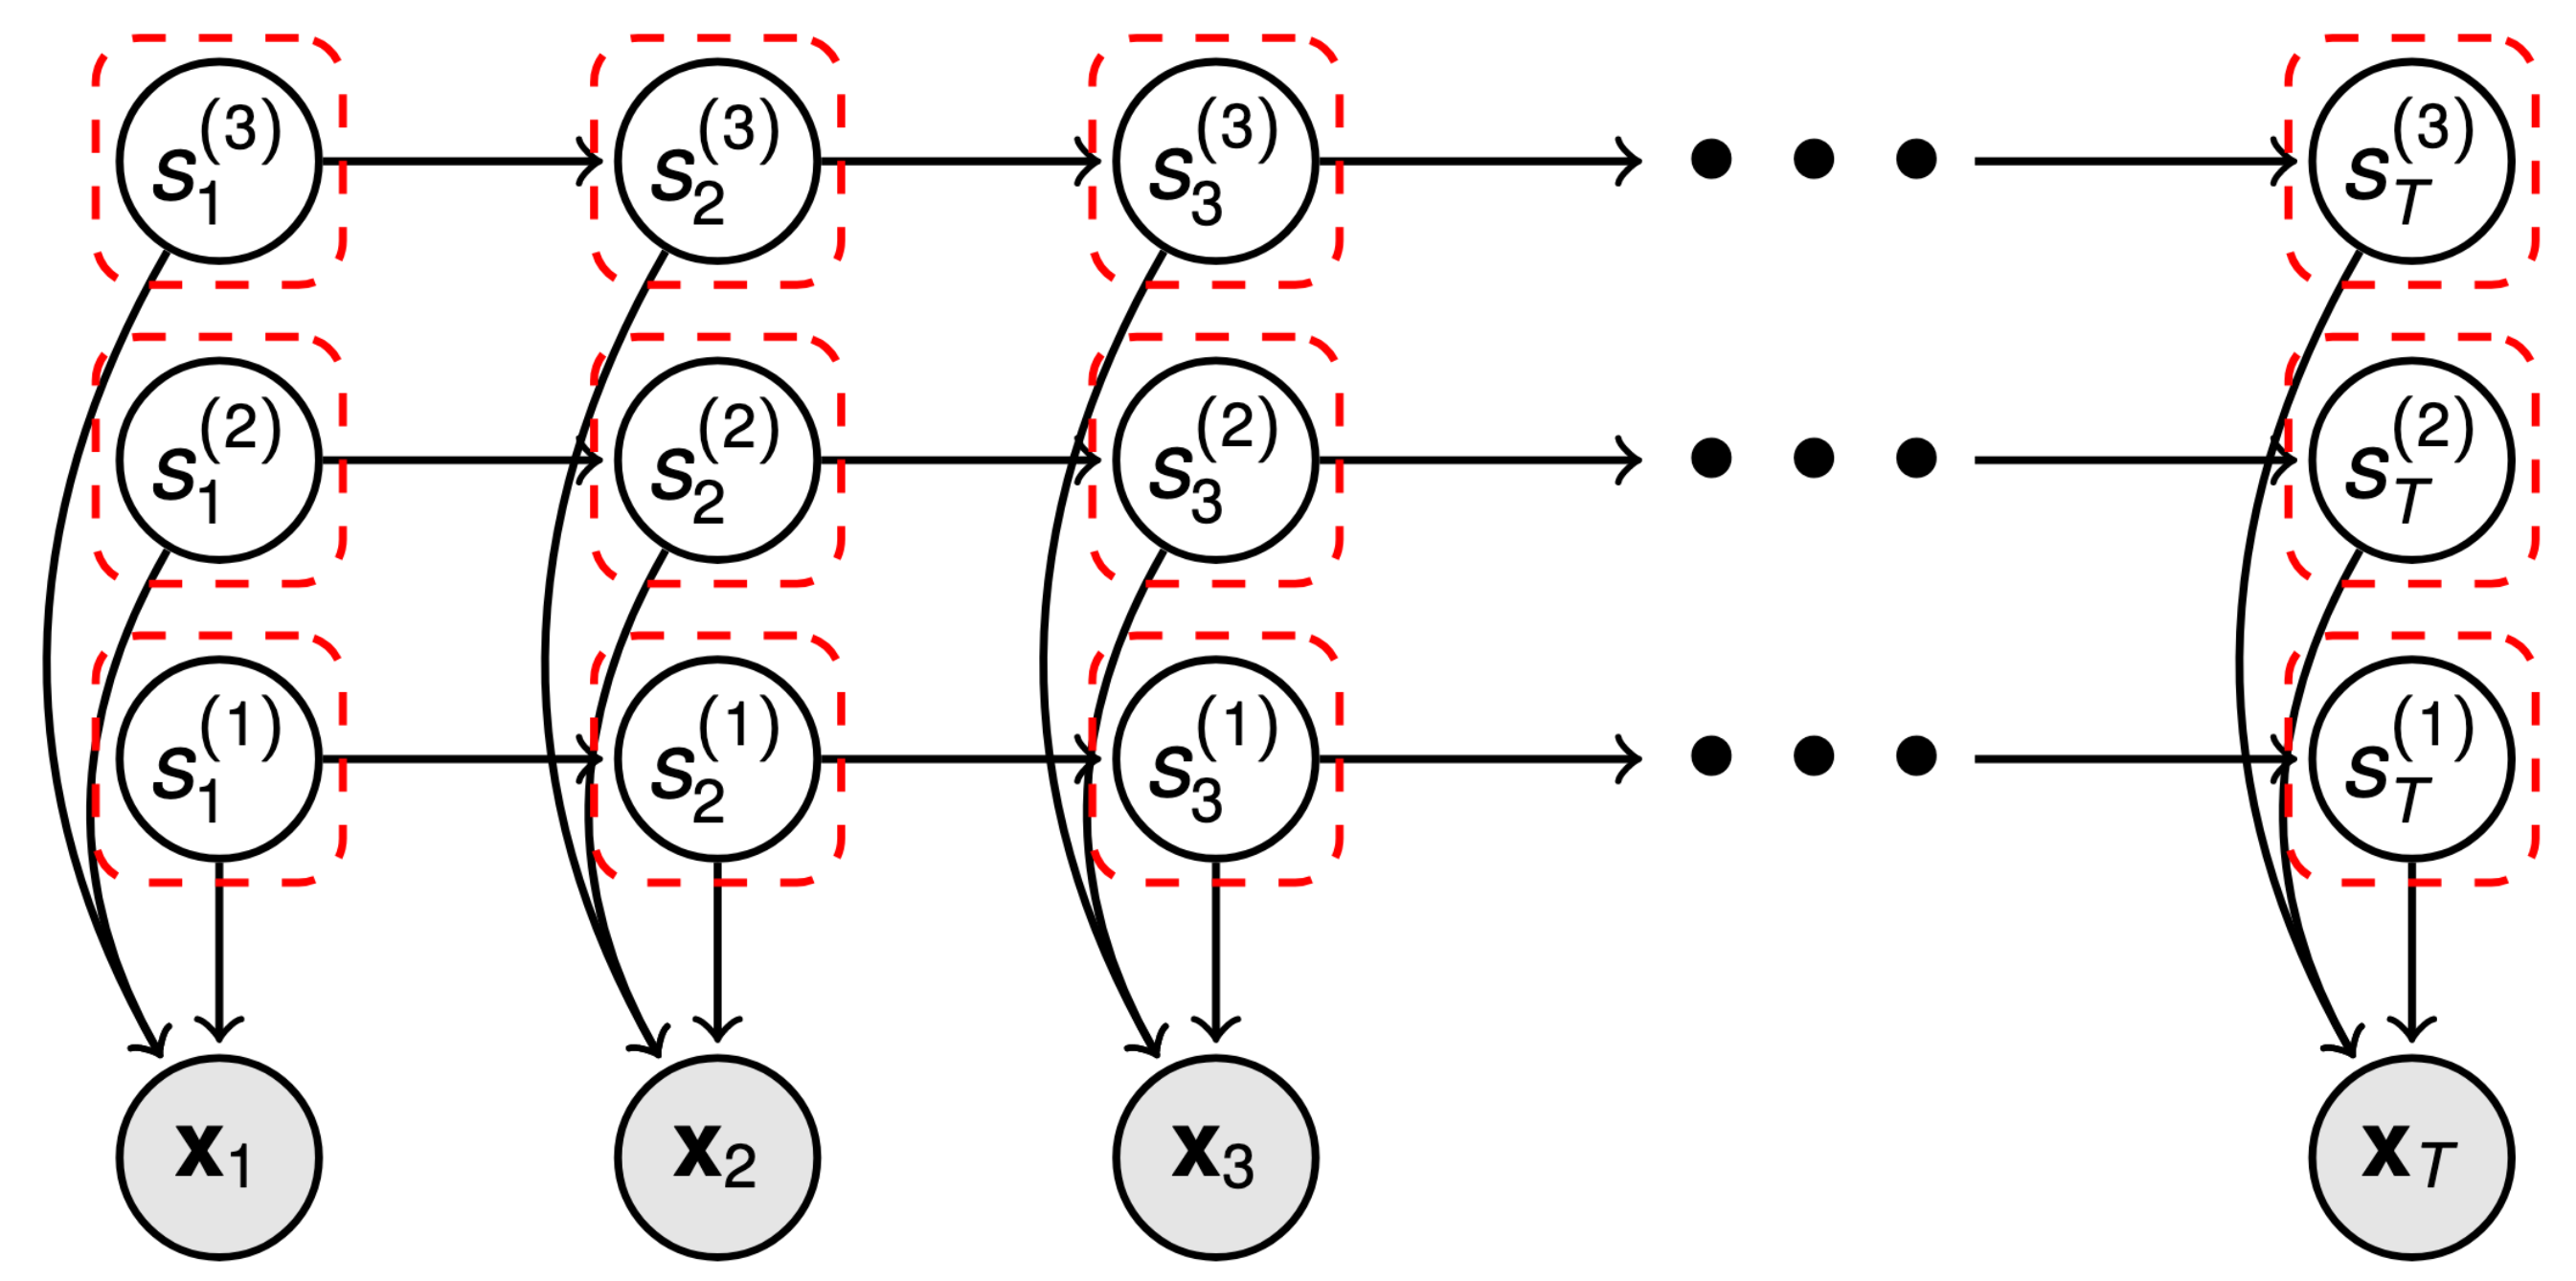
\includegraphics[width=8cm]{img/img12.png}
    \end{figure}  
    We consider the following inference with the factorization $\prod_{m,t}q^m_t(s^m_t)$, and so we have:
    \begin{equation*}
    \begin{aligned}
        q^{(m)}_t\bracka{s^{(m)}_t} &\propto \exp\brackd{ \log P\bracka{s^{1:M}_{1:T}, x_{1:T}} }_{\prod_{\neg(m, t)} q^{m'}_{t'}(s^{m'}_{t'}) } \\
        &=\exp\brackd{\sum_{\mu=1}^M\sum_{\tau=1}^T \log P(s^\mu_\tau | s^\mu_{\tau-1}) + \sum^T_{\tau=1}\log P(x_\tau | s^{1:M}_\tau) }_{\prod_{\neg(m, t)} q^{m'}_{t'}(s^{m'}_{t'}) } \\
    \end{aligned}
    \end{equation*}
    We can show that this is propotional to the following:
    \begin{equation*}
        \exp\Big[ \underbrace{\brackd{\log P(s^m_t | s^m_{t-1})}_{q^m_{t-1}} + \brackd{\log P(x_t | s^{1:M}_t)}_{\prod_{\neg m}q^{m'}_t}}_{\alpha^m_t(i)} + \underbrace{\brackd{\log P(s^m_{t-1} | s^m_t)}_{q^m_{t+1}}}_{\beta^m_i(i)} \Big]
    \end{equation*}
    Where we have the following variables (as we have the same message passing algorithm):
    \begin{equation*}
    \begin{aligned}
        &\alpha^m_t(i)\propto \exp\brackb{\sum_j \log \Phi^m_{ji}q^m_{t-1}(j)}\cdot\exp\brackb{\brackd{\log A_i(x_t)}_{q^{\neg m}_t} } \\
        &\beta^m_t(i)\propto \exp\brackb{\sum_j \log \Phi^m_{ij}q^m_{t+1}(j)}
    \end{aligned}
    \end{equation*}
    The update only depends on the immediate neighbours in chain. The chain couple only through joint output. It has multiple passes and message depends on (approximate) marginal. Finally, the evidence doesn't appear explicitly in backward message. 
\end{remark}

\begin{remark}{\textbf{(Difference Factored Variational Inference)}}
    Consider the difference kind of factorization:
    \begin{equation*}
        q(s^{1:M}_{1:T}) = \prod_m q^m(s^m_{1:T})
    \end{equation*}
    This gives us the following graphical model:
    \begin{equation*}
    \begin{aligned}
        q^{(m)}(s^m_{1:T}) &\propto \exp\bracka{\brackd{\log p\bracka{s^{1:M}_{1:T}, x_{1:T}}}_{\prod_{\neg m}q^{m'}(s^{m'}_{1:T})}} \\
        &= \exp\brackb{ \sum_{t=1}^T \log P(s^m_t | s^m_{t-1}) + \sum_{t=1}^T \brackd{\log P(x_t | s_t^{1:M})}_{\prod_{\neg m}q^{m'}(s^{m'}_t)} }
    \end{aligned}
    \end{equation*}
    Please note that this is similar to standard HMM joint with a modified likelihood term, where we cycle through multiple forward-backward pass updating likelihood terms each time. 
\end{remark}

\begin{remark}{\textbf{(Message on Arbitrary Graph)}}
    Consider DAG, where we have, the following:
    \begin{equation*}
        P(\mathcal{X}, \mathcal{Z}) = \prod_k P(\mathcal{V}_k | \operatorname{Pa}(\mathcal{V}_k))
    \end{equation*}
    We let $q(\mathcal{Z}) = \prod_i q_i(\mathcal{Z})$ for disjoint set $\brackc{\mathcal{Z}_i}$. We have the following VE update:
    \begin{equation*}
        q^*_i(\mathcal{Z}_i) \propto \exp\bracka{\brackd{\log P(\mathcal{X}, \mathcal{Z})}_{q_{\neg i}(\mathcal{Z})} }
    \end{equation*}
    Then, we have the following:
    \begin{equation*}
    \begin{aligned}
        \log q^*_i(\mathcal{Z}_i) &= \brackd{\sum_k P(\mathcal{V}_k | \operatorname{Pa}(\mathcal{V}_k))}_{q_{\neg i}(\mathcal{Z})} + \const \\
        &= \sum_{j\in\mathcal{Z}_i} \brackd{ \log P(\mathcal{Z}_j | \operatorname{Pa}(\mathcal{Z}_j)) }_{q_{\neg i}(\mathcal{Z})} + \sum_{j\in\operatorname{ch}(\mathcal{Z}_i)}\brackd{\log P(V_j | \operatorname{Pa}(V_j))}_{q_{\neg i}(\mathcal{Z})} + \const
    \end{aligned}
    \end{equation*}
    Each node receives message from its markov boundary: parent/children/parent of children (all neighbours in the corresponding graphs).
\end{remark}

\begin{remark}{\textbf{(Non-Factored Variational Model)}}
    The term variational approximation is used whenever a bound on likelihood is optimized, but not necessary be tight, as we have:
    \begin{itemize}
        \item Closed form update in special case. 
        \item Numerical or sampling based computation of expectation.
        \item Recognition Network or amortization to approximate variational parameter. 
        \item No free energy based bound on the likelihood. 
        \item We can perform MAP estimate or zero-temperature EM as parametric form of variational infernece. 
    \end{itemize}
\end{remark}

\begin{proposition}{\textbf{(Variational Bayes)}}
    We can consider performing the same for integral over parameter in other to bound the log-marginal likelihood or evidence:
    \begin{equation*}
    \begin{aligned}
        \log P(\mathcal{X} |\mathcal{M}) &= \log \iint P(\mathcal{Z},\mathcal{X} | \theta, \mathcal{M}) P(\theta|\mathcal{M})\dby\mathcal{Z}\dby\theta \\
        &= \max_{\mathcal{Q}}\iint Q(\mathcal{Z}, \theta) \log \frac{P(\mathcal{X},\mathcal{Z},\theta|\mathcal{M})}{Q(\mathcal{Z}, \theta)}\dby\mathcal{Z}\dby\theta \\
        &\ge \max_{Q_\mathcal{Z},Q_\mathcal{X}} \iint Q_\mathcal{Z}(\mathcal{Z}) Q_\theta(\theta) \log \frac{P(\mathcal{X},\mathcal{Z},\theta|\mathcal{M})}{Q_\mathcal{Z}(\mathcal{Z}) Q_\theta(\theta)}\dby\mathcal{Z}\dby\theta = \max_{Q_\mathcal{Z},Q_\mathcal{X}}  \mathcal{F}(Q_\mathcal{Z}, Q_\theta) \\
    \end{aligned}
    \end{equation*}
    The second equality comes from the Jensen's inequality bound being tight. This leads to variational Bayesian EM algorithm with free energy being $\mathcal{F}(Q_\mathcal{Z}, Q_\theta)$:
    \begin{equation*}
    \begin{aligned}
        &Q^*_\mathcal{Z}(\mathcal{Z}) \propto \exp\brackd{\log P(\mathcal{Z}, \mathcal{X} | \theta)}_{Q_\theta(\theta)} \\
        &Q^*_\theta(\theta) \propto P(\theta)\exp\brackd{\log (\mathcal{Z}, \mathcal{X}|\theta)}_{Q_\mathcal{Z}(\theta)}
    \end{aligned}
    \end{equation*}
\end{proposition}
\begin{proof}
    The maximizing $\mathcal{F}$ is the same as minimizing KL-divergence between the approximate posterior $Q(\mathcal{Z})Q(\theta)$ and the true posterior $P(\theta,\mathcal{Z}|\mathcal{X})$ as we have:
    \begin{equation*}
    \begin{aligned}
        \log P(\mathcal{X}) - \mathcal{F}(Q_\mathcal{Z}, Q_\theta) &= \iint Q_\mathcal{Z}(\mathcal{Z})Q_\theta(\theta)\log P(\mathcal{X})\dby\mathcal{Z}\dby\theta - \iint Q_\mathcal{Z}(\mathcal{Z}) Q_\theta(\theta) \log \frac{P(\mathcal{X},\mathcal{Z},\theta|\mathcal{M})}{Q_\mathcal{Z}(\mathcal{Z}) Q_\theta(\theta)}\dby\mathcal{Z}\dby\theta \\
        &= \iint Q_\mathcal{Z}(\mathcal{Z}) Q_\theta(\theta) \log \frac{Q_\mathcal{Z}(\mathcal{Z}) Q_\theta(\theta)}{P(\mathcal{Z},\theta|\mathcal{X}, \mathcal{M})}\dby\mathcal{Z}\dby\theta = \operatorname{KL}(Q\| P)
    \end{aligned}
    \end{equation*}
\end{proof}

\begin{remark}{\textbf{(Conjugate Exponential)}}
    Let's consider the conjugate exponential model on latent variable:
    \begin{itemize}
        \item \emph{Condition 1}: Consider the joint probability over variables in exponential family:
        \begin{equation*}
            P(\mathcal{Z},\mathcal{X}|\boldsymbol \theta) = f(\mathcal{X},\mathcal{Z})g(\boldsymbol \theta)\exp\brackc{\boldsymbol \phi(\boldsymbol \theta)^T\boldsymbol T(\mathcal{Z}, \mathcal{X})} 
        \end{equation*}
        \item \emph{Condition 2}: The joint over parameter is conjugate to this joint probability:
        \begin{equation*}
            P(\boldsymbol \theta | \nu, \boldsymbol \tau) = h(\nu, \boldsymbol \tau)g(\boldsymbol \theta)^\nu \exp\brackc{\boldsymbol \phi(\boldsymbol \theta)^T\boldsymbol \tau}
        \end{equation*}
        where $\nu$ and $\boldsymbol \tau$ on the prior and we can see them as number of pseudo-observations and values of pseudo-observations, respectively.
    \end{itemize}
\end{remark}

\begin{remark}{\textbf{(Conjugate Exponential VB)}}
    Given a iid set $\mathcal{D} = \brackc{\boldsymbol x_1,\boldsymbol x_2,\dots,\boldsymbol x_n}$  if the model is conjugate exponential then we have. $Q_\theta(\boldsymbol \theta)$ is also conjugate, as we have:
    \begin{equation*}
    \begin{aligned}
        Q_\theta(\boldsymbol \theta) &\propto P(\boldsymbol \theta)\exp\brackd{\sum_i \log P(\mathcal{Z}_i, \mathcal{X}_i | \boldsymbol \theta)}_{Q_\mathcal{Z}(\mathcal{Z})} \\
        &= h(\nu, \boldsymbol \tau)g(\boldsymbol \theta)^\nu \exp\bracka{\boldsymbol \phi(\boldsymbol \theta)^T\boldsymbol \tau} g(\boldsymbol \theta)^n \exp\bracka{ \brackd{ \log f(\mathcal{X}, \mathcal{Z}) + \sum^n_{i=1} \boldsymbol \phi(\boldsymbol \theta)^T\boldsymbol T(\boldsymbol z_i, \boldsymbol x_i) }_{Q_\mathcal{Z}} } \\
        &\propto h(\tilde{\nu}, \tilde{\boldsymbol \tau})g(\boldsymbol \theta)^{\nu + n} \exp\bracka{ \boldsymbol \phi(\boldsymbol \theta)^T \bracka{ \boldsymbol \tau + \brackd{\sum^n_{i=1} \boldsymbol T(\boldsymbol z_i, \boldsymbol x_i) }_{Q_\mathcal{Z}} } } = h(\tilde{\nu}, \tilde{\boldsymbol \tau})g(\boldsymbol \theta)^{\tilde{\nu}} \exp\bracka{ \boldsymbol \phi(\boldsymbol \theta)^T \tilde{\boldsymbol\tau} }
    \end{aligned}
    \end{equation*}
    we can set $\tilde{\nu} = \nu + n$ and $\tilde{\boldsymbol \tau} = \tau + \sum_i \brackd{\boldsymbol T(\boldsymbol z_i, \boldsymbol x_i)}_{Q_\mathcal{Z}}$
\end{remark}

\begin{remark}{\textbf{(Factorized EM)}}
    We have the following factorized model as we have $Q_\mathcal{Z}(\mathcal{Z}) = \prod^n_{i=1}Q_{\mathcal{Z}_i}(\mathcal{Z}_i)$ (over the dataset). It has the same form as regular E-step of regular EM, where we have:
    \begin{equation*}
    \begin{aligned}
        Q_{\mathcal{Z}_i}(\mathcal{Z}_i) &\propto \exp\bracka{ \brackd{\log P(\boldsymbol z_i, \boldsymbol x_i)}_{Q_\theta} } \\
        &\propto f(\boldsymbol z_i, \boldsymbol x_i)\exp\brackc{ \brackd{\boldsymbol \phi(\boldsymbol \theta)}^T_{Q_\theta} \boldsymbol T(\boldsymbol z_i,\boldsymbol x_i) } \\
        &= P(\boldsymbol z_i | \boldsymbol x_i, \tilde{\boldsymbol \phi}(\boldsymbol \theta))
    \end{aligned}
    \end{equation*} 
    where the natural parameter $\tilde{\boldsymbol \phi}(\boldsymbol \theta) = \brackd{\boldsymbol \phi(\boldsymbol \theta)}_{Q_\theta}$, where the inference is unchanged to regular EM.
\end{remark}

\begin{remark}{\textbf{(Comparison Between EM for MAP estimation and Variational Baysian EM)}} Let's compare the differences between the $2$ algorithms:
    \begin{figure}[H]
        \centering
        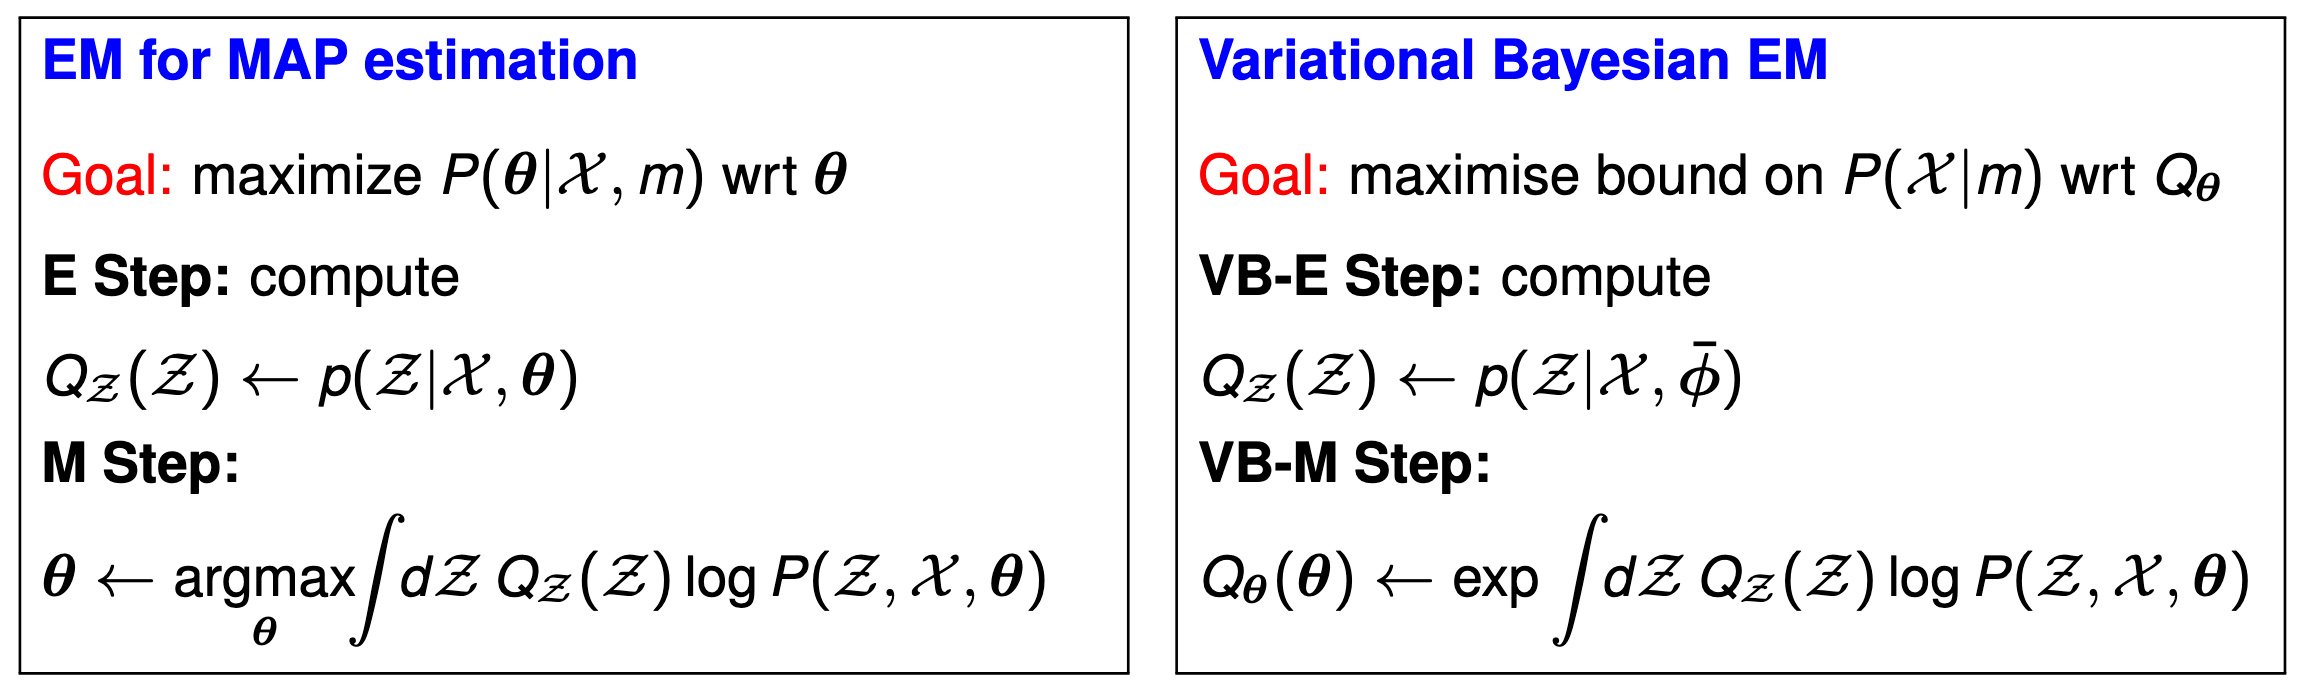
\includegraphics[width=12cm]{img/img13.png}
    \end{figure}  
    The following are the feature of VB, as we have:
    \begin{itemize}
        \item It reduces to EM if we set $Q_\theta(\boldsymbol \theta) = \delta(\boldsymbol \theta-\boldsymbol \theta^*)$
        \item $\mathcal{F}_m$ increase monotonically and interpolate the model complexity penalty. 
        \item We have analytical parameter distribution but we don't have to contraint to Gaussian.
        \item VB-E step has the same complexity as E-step. 
        \item We can use junction tee, belief propagatio, kalman filter algorithm in VB E-step of VB-EM but we have to use the expected natural parameter $\tilde{\boldsymbol \phi}$. 
    \end{itemize}
\end{remark}

\begin{remark}{\textbf{(VB and Model Classification)}}
    VB-EM gives us the approximate posterior $Q_\theta$ over the model parameter:
    \begin{itemize}
        \item It also gives us the lower bound on the model estimate as we have:
        \begin{equation*}
            \max\mathcal{F}_M(Q_\mathcal{Z}, Q_\theta) \le P(\mathcal{D}|\mathcal{M})
        \end{equation*}
        \item These lower bound can be compared amongts model to find the right out. However, if we consider continuous domain of model that is specified by the hyperparameter $\eta$, then VB free energy depends on parameter
        \begin{equation*}
            \mathcal{F}(Q_\mathcal{Z}, Q_\theta,\eta) = \iint Q_\mathcal{Z}(\mathcal{Z})Q_\theta(\boldsymbol \theta) \log \frac{P(\mathcal{X}, \mathcal{Z}, \boldsymbol \theta | \eta)}{Q_\mathcal{Z}(\mathcal{Z})Q_\theta(\boldsymbol \theta)}  \dby \mathcal{Z}\dby\boldsymbol \theta \le P(\mathcal{X}|\eta)
        \end{equation*}
        Hyperparameter-M step maximizes the current bound with respected to $\eta$:
        \begin{equation*}
            \eta \leftarrow \argmax{\eta} \iint Q_\mathcal{Z}(\mathcal{Z})Q_\theta(\boldsymbol \theta) \log P(\mathcal{X}, \mathcal{Z}, \boldsymbol \theta | \eta) \dby \mathcal{Z}\dby\boldsymbol \theta
        \end{equation*}
    \end{itemize}
\end{remark}

\begin{remark}{\textbf{(ARD for Unsupervised Learning)}}
    The hyperparameter method to select a useful input regression. This is similar idea with variational Bayes method that can learn a latent dimension. Consider the factor analysis:
    \begin{equation*}
        \boldsymbol x \sim \mathcal{N}(\boldsymbol \Lambda\boldsymbol z, \boldsymbol \Psi)
    \end{equation*}
    where $\boldsymbol z \sim \mathcal{N}(\boldsymbol 0, \boldsymbol I)$ with column-wise prior to be $\boldsymbol \Lambda_{:i}\sim \mathcal{N}(\boldsymbol 0, \alpha_i^{-1}\boldsymbol I)$. Then the VB free-energy is given by:
    \begin{equation*}
        \mathcal{F}\Big( Q_\mathcal{Z}(\mathcal{Z}), Q_\Lambda(\boldsymbol \Lambda), \boldsymbol \Psi, \boldsymbol \alpha \Big) = \Big\langle \log P(\mathcal{X}, \mathcal{Z} | \boldsymbol \Lambda, \boldsymbol \Psi) + \log P(\boldsymbol \Lambda | \boldsymbol \alpha) + \log P(\boldsymbol \Psi) \Big\rangle_{Q_\mathcal{Z}(\mathcal{Z})Q_\Lambda(\boldsymbol \Lambda)} + \const
    \end{equation*}
    We require the hyperparameter optimization require us $\boldsymbol \alpha \leftarrow \arg\max\brackd{\log P(\boldsymbol \Lambda | \boldsymbol \alpha)}_{Q_\Lambda}$. Now we obtain the following optimization:
    \begin{itemize}
        \item Now, $Q_\Lambda$ is Gaussian with the same form as linear regression but with expected moment of $\boldsymbol z$ instead of the input. 
        \item The optimization with respected to the distribution $\boldsymbol \Psi$ and $\boldsymbol \alpha$ will cause some $\alpha_i$ to diverge as in regression ARD. 
        \item Same as selecting relevant latent dimension, effectively learning the dimension of latent variable.
    \end{itemize}
\end{remark}

\begin{remark}{\textbf{(Problem with GP + Solution)}}
    Given the GP prediction, we have:
    \begin{equation*}
        y' | \boldsymbol X, \boldsymbol Y, \boldsymbol x \sim \mathcal{GP}( \boldsymbol K_{xX}(\boldsymbol K_{XX} + \sigma^2\boldsymbol I)^{-1} \boldsymbol Y, \ \boldsymbol K_{xx} - \boldsymbol K_{xX}(\boldsymbol K_{XX} + \sigma^2\boldsymbol I)^{-1}\boldsymbol K_{Xx} + \sigma^2 )
    \end{equation*} 
    The evidence (for learning the kernel hyperparameter) to be:
    \begin{equation*}
        \log P(\boldsymbol Y | \boldsymbol X) = -\frac{1}{2}\log\abs{2\pi(\boldsymbol K_{XX} + \sigma^2\boldsymbol I)}^{-1/2} \exp\bracka{-\frac{1}{2} \boldsymbol Y^T(\boldsymbol K_{XX} + \sigma^2\boldsymbol I)^{-1}\boldsymbol Y }
    \end{equation*}
    Computing this require inverting $N\times N$ matrix with has the time complexity of $\mathcal{O}(K^3)$. We consider the smaller set of possible fictious measurement $\boldsymbol U$ at input $\boldsymbol Z$ such that:
    \begin{equation*}
        P(y' | \boldsymbol Z, \boldsymbol U, \boldsymbol x') \approx P(y' | \boldsymbol X, \boldsymbol Y, \boldsymbol x')
    \end{equation*}
    Write $\boldsymbol F$ for the smooth GP function that underlie $\boldsymbol Y\sim\mathcal{N}(\boldsymbol F, \sigma^2I)$. Introduce the measurement $\boldsymbol U$ at input $\boldsymbol Z$, as the likelihood can be written as:
    \begin{equation*}
    \begin{aligned}
        P(\boldsymbol Y | \boldsymbol X) &= \iint P(\boldsymbol Y, \boldsymbol F, \boldsymbol U | \boldsymbol X, \boldsymbol Z) \dby \boldsymbol F\dby \boldsymbol U \\
        &= \iint P(\boldsymbol Y|\boldsymbol F)P(\boldsymbol F | \boldsymbol U, \boldsymbol X, \boldsymbol Z)P(\boldsymbol U | \boldsymbol Z)\dby \boldsymbol F\dby \boldsymbol U
    \end{aligned}
    \end{equation*}
\end{remark}

\begin{remark}{\textbf{(Free-Energy)}}
    As we have $\boldsymbol F$ and $\boldsymbol U$ to be the latent variable, we introduce the variational distribution $q(\boldsymbol F, \boldsymbol U)$ to be:
    \begin{equation*}
        \mathcal{F}(q(\boldsymbol F, \boldsymbol U), \theta) = \brackd{\log\frac{P(\boldsymbol Y|\boldsymbol F)P(\boldsymbol F | \boldsymbol U, \boldsymbol X, \boldsymbol Z)P(\boldsymbol U | \boldsymbol Z)}{q(\boldsymbol F, \boldsymbol U)}}_{q(\boldsymbol F, \boldsymbol U)}
    \end{equation*}
    Consider the variational distribution of the latent to be $q(\boldsymbol F, \boldsymbol U) = P(\boldsymbol F | \boldsymbol U, \boldsymbol X, \boldsymbol Z)q(\boldsymbol U)$. We fix $\boldsymbol F | \boldsymbol U$ with reference to $\boldsymbol U$ to make the information about $\boldsymbol Y$ is compressed to $q(\boldsymbol U)$, which we have:
    \begin{equation*}
    \begin{aligned}
        \mathcal{F}(q(\boldsymbol F, \boldsymbol U), \theta, \boldsymbol Z) &= \brackd{\log \frac{P(\boldsymbol Y|\boldsymbol F)P(\boldsymbol F | \boldsymbol U, \boldsymbol X, \boldsymbol Z)P(\boldsymbol U | \boldsymbol Z)}{P(\boldsymbol F | \boldsymbol U, \boldsymbol X, \boldsymbol Z)q(\boldsymbol U)}}_{P(\boldsymbol F | \boldsymbol U, \boldsymbol X, \boldsymbol Z)q(\boldsymbol U)} \\
        &= \brackd{\log \frac{P(\boldsymbol Y|\boldsymbol F)P(\boldsymbol U | \boldsymbol Z)}{q(\boldsymbol U)}}_{P(\boldsymbol F | \boldsymbol U, \boldsymbol X, \boldsymbol Z)q(\boldsymbol U)} \\
        &= \brackd{\brackd{\log P(\boldsymbol Y|\boldsymbol F)}_{P(\boldsymbol F | \boldsymbol U, \boldsymbol X, \boldsymbol Z) } + \log P(\boldsymbol U | \boldsymbol Z) - q(\boldsymbol U)}_{q(\boldsymbol U)}
    \end{aligned}
    \end{equation*}
    Let's consider the inner expectation, which we can use the Gaussian process results (without noise on $\boldsymbol F$):
    \begin{equation*}
    \begin{aligned}
        \brackd{\log P(\boldsymbol Y|\boldsymbol F)}_{P(\boldsymbol F | \boldsymbol U, \boldsymbol X, \boldsymbol Z) } &= \brackd{-\frac{1}{2}\log\abs{2\pi\sigma^2\boldsymbol I} - \frac{1}{2\sigma^2}\operatorname{Tr}\brackb{(\boldsymbol Y-\boldsymbol F)(\boldsymbol Y-\boldsymbol F)^T}}_{P(\boldsymbol F | \boldsymbol Y)} \\
        &= -\frac{1}{2}\log \abs{2\pi\sigma^2\boldsymbol I} - \frac{1}{2\sigma^2}\operatorname{Tr}\brackb{ \bracka{\boldsymbol Y - \brackd{\boldsymbol F}_{P(\boldsymbol F | \boldsymbol Y)}} \bracka{\boldsymbol Y - \brackd{\boldsymbol F}_{P(\boldsymbol F|\boldsymbol Y)}}^T } - \frac{1}{2\sigma^2}\operatorname{Tr}\brackb{\boldsymbol \Sigma_{F|U}} \\
        &= \log \mathcal{N}(\boldsymbol Y | \boldsymbol K_{XZ}\boldsymbol K^{-1}_{ZZ}\boldsymbol U, \sigma^2\boldsymbol I) - \frac{1}{2\sigma^2}\operatorname{Tr}[\boldsymbol K_{XX} - \boldsymbol K_{XZ}\boldsymbol K_{ZZ}^{-1}\boldsymbol K_{ZX}]
    \end{aligned}
    \end{equation*}
    This gives us the following free energy function:
    \begin{equation*}
        \mathcal{F}(q(\boldsymbol U), \boldsymbol \theta, \boldsymbol Z) = \brackd{\log \frac{\mathcal{N}(\boldsymbol Y | \boldsymbol K_{XZ}\boldsymbol K^{-1}_{ZZ} \boldsymbol U, \ \sigma^2\boldsymbol I) P(\boldsymbol U | \boldsymbol Z) }{ q(\boldsymbol U) }}_{q(\boldsymbol U)} - \frac{1}{2\sigma^2}\operatorname{Tr}[\boldsymbol K_{XX} - \boldsymbol K_{XZ}\boldsymbol K_{ZZ}^{-1}\boldsymbol K_{ZX}]
    \end{equation*}
    Now, we can see that the expectation is free energy of PPCA-like model with the latent to be $\boldsymbol U \sim \mathcal{N}(\boldsymbol 0, \boldsymbol K_{ZZ})$, with the following linear Gaussian model $p(\boldsymbol K_{XZ}\boldsymbol K_{ZZ}^{-1} \boldsymbol U, \sigma^2 \boldsymbol I)$, thusm we have the following free energy:
    \begin{equation*}
    \begin{aligned}
        \mathcal{F}(q^*(\boldsymbol U), \boldsymbol \theta, \boldsymbol Z) 
        &= \log \mathcal{N}(\boldsymbol Y | \boldsymbol 0, \boldsymbol K_{XZ}\boldsymbol K_{ZZ}^{-1}\boldsymbol K_{ZZ}\boldsymbol K_{ZZ}^{-1}\boldsymbol K_{ZX} + \sigma^2\boldsymbol I) - \frac{1}{2\sigma^2}\operatorname{Tr}[\boldsymbol K_{XX} - \boldsymbol K_{XZ}\boldsymbol K_{ZZ}^{-1}\boldsymbol K_{ZX}] \\
        &= \log \mathcal{N}(\boldsymbol Y | \boldsymbol 0, \boldsymbol K_{XZ}\boldsymbol K_{ZZ}^{-1}\boldsymbol K_{ZX} + \sigma^2\boldsymbol I) - \frac{1}{2\sigma^2}\operatorname{Tr}[\boldsymbol K_{XX} - \boldsymbol K_{XZ}\boldsymbol K_{ZZ}^{-1}\boldsymbol K_{ZX}] \\
    \end{aligned}
    \end{equation*}
    We can now optimize the free energy numerically with respect to $\boldsymbol \theta$ and $\boldsymbol Z$ to adjust GP prior and quality of variational approximation. 
\end{remark}

\begin{remark}
    If $\boldsymbol X$ is unobserved, then assume that $q(\boldsymbol X, \boldsymbol F, \boldsymbol U) = q(\boldsymbol X)P(\boldsymbol F, \boldsymbol X, \boldsymbol U)q(\boldsymbol U)$ then we have the free energy to be:
    \begin{equation*}
        \mathcal{F} = \brackd{\log P(\boldsymbol Y, \boldsymbol F, \boldsymbol U | \boldsymbol X)+ \log P(\boldsymbol X)}_{q(\boldsymbol U)q(\boldsymbol X)}
    \end{equation*}
    which can be simplifed to tractable components in similar way as above. 
\end{remark}
